\documentclass[tikz,border=10pt]{standalone}

\usepackage{tikz}

\begin{document}

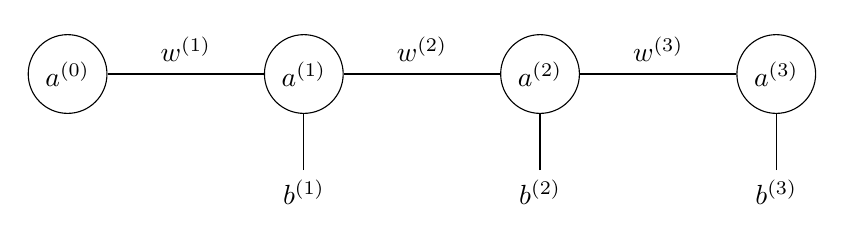
\begin{tikzpicture}[
    neuron/.style={circle, draw, minimum size=1cm}
]

    \node[neuron] (N1) at (0, 0) {$a^{(0)}$};
    \node[neuron] (N2) at (3, 0) {$a^{(1)}$};
    \node[neuron] (N3) at (6, 0) {$a^{(2)}$};
    \node[neuron] (N4) at (9, 0) {$a^{(3)}$};

    \node (B1) at (3, -1.5) {$b^{(1)}$};
    \node (B2) at (6, -1.5) {$b^{(2)}$};
    \node (B3) at (9, -1.5) {$b^{(3)}$};

    \draw (N1) -- node[midway, above, yshift=1pt] {$w^{(1)}$} (N2);
    \draw (N2) -- node[midway, above, yshift=1pt] {$w^{(2)}$} (N3);
    \draw (N3) -- node[midway, above, yshift=1pt] {$w^{(3)}$} (N4);

    \draw (B1) -- (N2);
    \draw (B2) -- (N3);
    \draw (B3) -- (N4);
\end{tikzpicture}

\end{document}
